\chapter{Planificación del proyecto}\label{cap:planificacion}

\section{Cronograma del proyecto}

Antes del comienzo del desarrollo del proyecto, se realizó una planificación inicial que incluía la definición de los sprints y las tareas a realizar en cada uno de ellos de manera general, definiendo hitos, no tareas específicas. Esta planificación se ha seguido a lo largo del desarrollo, aunque ha habido ajustes en función de los avances y los resultados obtenidos.

La realización del cronograma se ha llevado a cabo haciendo uso de la herramienta \textbf{GantPRO}\cite{webGanttPro}, que permite la creación de diagramas de Gantt de manera sencilla y efectiva. A continuación, se presenta el diagrama de Gantt del proyecto, que muestra las diferentes fases y tareas a realizar en cada sprint.

\begin{figure}[ht!] 
    \centering 
    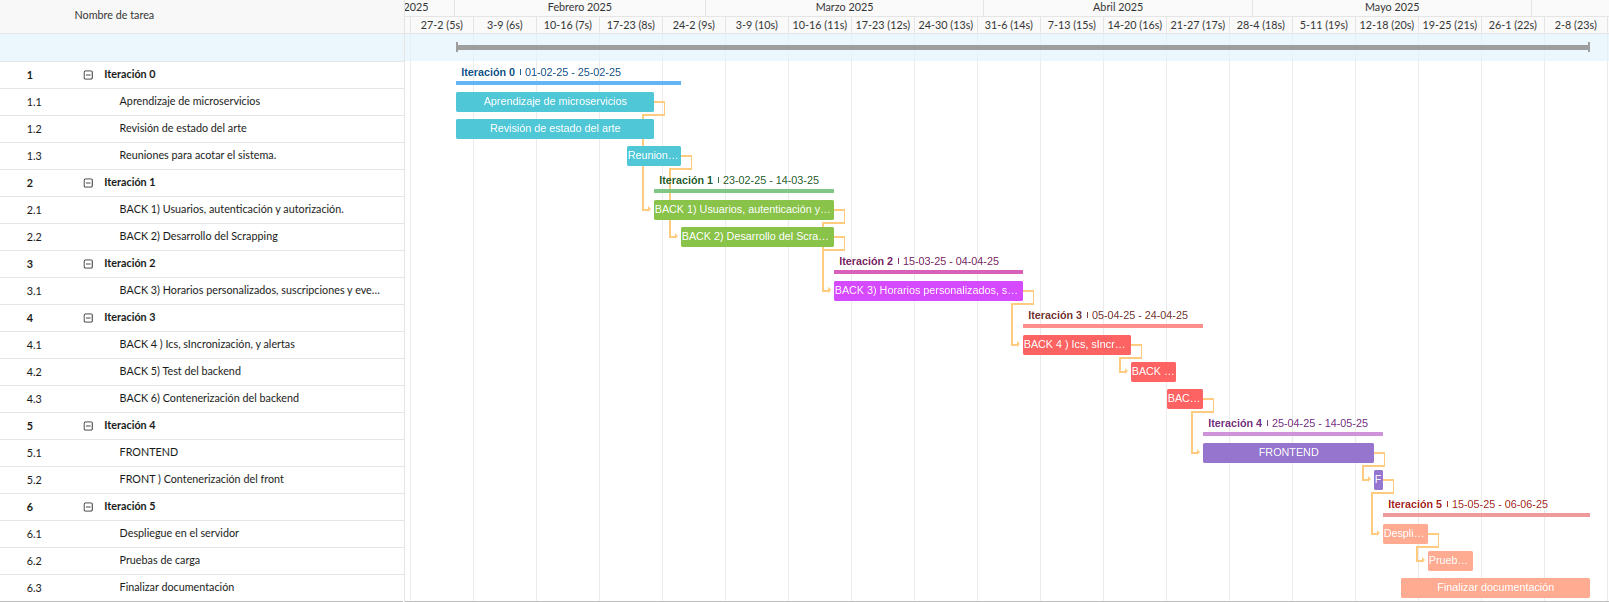
\includegraphics[width=1\textwidth]{figures/04_gantt.png}
    \caption{Gantt del proyecto.} 
    \label{gantt}
\end{figure}

El cronograma del proyecto se ha dividido en 5 sprints, cada uno con una duración de 3 semanas. Como se muestra en la figura \ref{gantt}, cada sprint ha tenido un conjunto de tareas generales a realizar, que se han ido completando a lo largo del desarrollo.

\begin{enumerate}
    \item \textbf{Sprint 0:} En este sprint se paraleliza por un lado el aprendizaje técnico acerca de microservicios, docker y el framework de desarrollo backend \textbf{Spring Boot}, a la vez que se acota el sistema y se recaban los requisitos iniciales del sistema.
    \item \textbf{Sprint 1:} En este sprint se comienza el desarrollo del backend implementando los servicios relativos a los usuarios, y la autenticación y autorización basadas en las credenciales de la UGR junto al servicio de mensajería (notificaciones). Además se implementa el scrapping de la we de ``Grados UGR'' para obtener los horarios de los grados.
    \item \textbf{Sprint 2:} En este sprint se continúa el backend implementando las funcionalidades relativas a suscripciones, horarios personalizados y creación de eventos.
    \item \textbf{Sprint 3:} En este sprint se desarrolla la parte del backend relacionada con generación de archivos ics, sincronización con sistemas de calendarios externos y alertas. Además se realizan tests y la contenerización del sistema.
    \item \textbf{Sprint 4:} En este sprint se desarrolla el frontend del sistema, implementando la interfaz de usuario y la comunicación con el backend.
    \item \textbf{Sprint 5:} En este último sprint se realiza el despliegue en el servidor de la UGR, se realizan pruebas de carga y se finaliza el proyecto para su entrega.
\end{enumerate}

En todos los sprints se realizarán además tareas de documentación y pruebas, además del seguimiento y registro de horas dedicadas a cada tarea.

\section{Metodología de desarrollo}
Para la gestión y desarrollo del proyecto, se ha optado por la metodología ágil \hyperlink{scrum}{Scrum}. Esta metodología se caracteriza por su enfoque iterativo e incremental, permitiendo una adaptación flexible a los cambios y una entrega temprana de valor.

\subsection{Roles y Responsabilidades en este Proyecto}

Dada la naturaleza individual de este proyecto, los roles tradicionales de Scrum se han adaptado de la siguiente manera:

\begin{itemize}
    \item \textbf{Equipo de Desarrollo y Scrum Master:} El autor de este TFG ha asumido ambos roles. Esto implica la responsabilidad de llevar a cabo el desarrollo del software, así como de facilitar el proceso Scrum, asegurando que se sigan las prácticas y principios de la metodología. Se ha encargado de la planificación, ejecución y revisión de cada sprint, así como de la identificación y resolución de impedimentos.
    \item \textbf{Product Owner:} El rol de Product Owner ha sido desempeñado tanto por el director del TFG, D. Juan Luis Jiménez Laredo, como por el autor del sistema. En esta función, ambos han sido los responsables de definir la visión del producto, priorizar el Backlog del Producto y asegurar que el desarrollo se alinee con las necesidades y expectativas del proyecto. Los dos participaron activamente en la definición de los requisitos y en la validación de los incrementos de software.
\end{itemize}

\subsection{Proceso Scrum Implementado}

El proceso Scrum se ha implementado siguiendo los siguientes pasos clave:

\begin{itemize}
    \item \textbf{\hyperlink{backlog}{Backlog} del Producto:} Se ha definido un Backlog del Producto inicial, compuesto por las funcionalidades y tareas necesarias para completar el TFG.
    \item \textbf{Sprints:} El desarrollo se ha dividido en 5 sprints de duración 3 semanas cada uno. Cada sprint ha tenido como objetivo la entrega de un incremento de software funcional y potencialmente entregable.
    \item \textbf{Planificación del Sprint:} Al inicio de cada sprint, se ha llevado a cabo una reunión de planificación en la que, junto con el Product Owner, se han seleccionado los elementos del Backlog del Producto que se abordarían durante el sprint. Se han estimado las tareas y se ha definido el Sprint Backlog.
    \item \textbf{Desarrollo del Sprint:} Durante el sprint, el autor ha trabajado en el desarrollo de las tareas asignadas, siguiendo las prácticas de desarrollo y asegurando la calidad del código.
    \item \textbf{Reunión Diaria (Daily Scrum):} Aunque adaptada a la naturaleza individual del proyecto, se ha realizado una reflexión diaria sobre el progreso, los impedimentos y las tareas a realizar. Esto ha permitido mantener un seguimiento constante del avance.
    \item \textbf{Revisión del Sprint (Sprint Review):} Al finalizar cada sprint, se ha llevado a cabo una revisión del sprint. Dado que el autor es también el equipo de desarrollo, esta revisión ha consistido en una \textbf{introspección personal y un análisis de los resultados del sprint}, evaluando las metas alcanzadas y el incremento de software desarrollado. Se ha realizado una autoevaluación del progreso y la calidad del trabajo.
    \item \textbf{Retrospectiva del Sprint (Sprint Retrospective):} La retrospectiva del sprint se ha realizado en colaboración con el Product Owner (D. Juan Luis Jiménez Laredo). En esta reunión, se ha analizado el sprint finalizado, identificando qué se ha hecho bien, qué se podría mejorar y qué acciones concretas se podrían implementar para el siguiente sprint. Esta colaboración ha permitido obtener una perspectiva externa y valiosa para la mejora continua del proceso.
\end{itemize}

\subsection{Gestión de Tareas y Seguimiento del Progreso}

Para la gestión de las tareas y el seguimiento del progreso del proyecto, se ha utilizado \textbf{GitHub Projects}. Esta herramienta ha permitido:

\begin{itemize}
    \item \textbf{Creación de Tableros por Sprint:} Se han configurado tableros de proyecto en GitHub Projects, utilizando las funcionalidades de \textbf{``Iteraciones''} para representar cada sprint. Esto ha facilitado la visualización del trabajo en curso para cada iteración.
    \item \textbf{Gestión del Estado de las Tareas:} Dentro de cada tablero de sprint, se han creado y gestionado las tareas individuales, asignándoles diferentes estados ( ``Backlog'', ``Todo'', ``In progress'', ``Testing'', ``Done''). Esto ha permitido un seguimiento visual del avance de cada tarea y del sprint en general.
    \item \textbf{Organización y Priorización:} GitHub Projects ha facilitado la organización de las tareas y su priorización dentro de cada sprint, alineándose con el Sprint Backlog definido.
    \item \textbf{Visualización de las tareas en el tiempo:} La herramienta ha permitido visualizar el progreso de las tareas en el tiempo a través de un roadmap, lo que ha facilitado la identificación de posibles retrasos y la toma de decisiones para ajustar el plan si es necesario.
\end{itemize}

\begin{figure}[H] 
    \centering 
    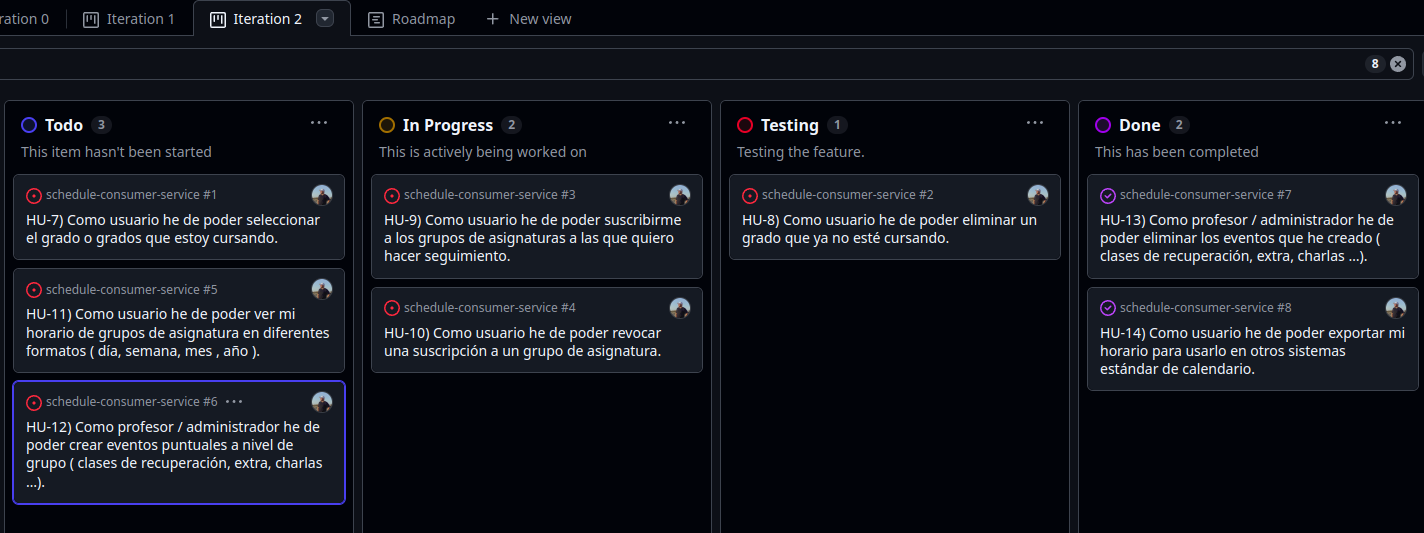
\includegraphics[width=1\textwidth]{figures/04_github_tablero.png}
    \caption{Tablero del 2º Sprint durante su desarrollo.} % Leyenda de la imagen
    \label{tablero_github} % Etiqueta para referenciar la imagen
\end{figure}

\begin{figure}[H] 
    \centering 
    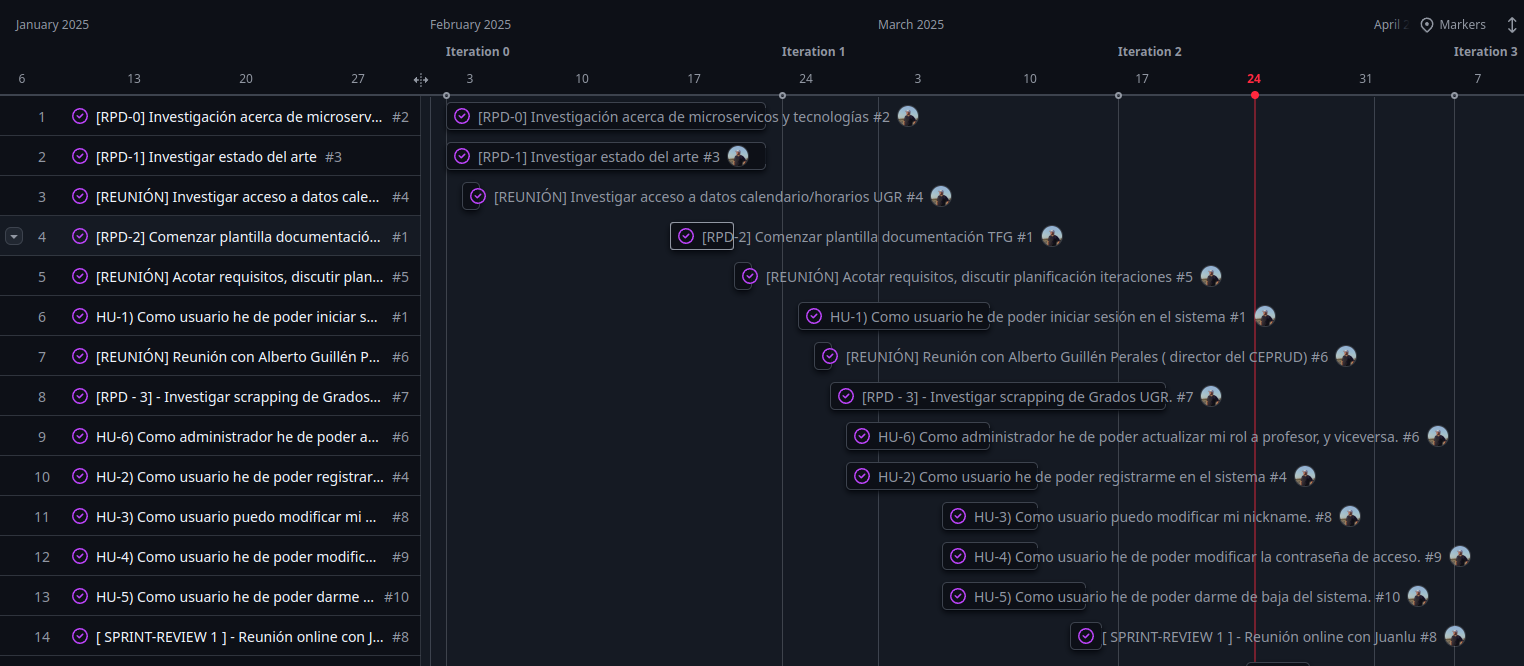
\includegraphics[width=1\textwidth]{figures/04_roadmap.png}
    \caption{Segmento del ''Roadmap'' del proyecto.} % Leyenda de la imagen
    \label{roadmap_github} % Etiqueta para referenciar la imagen
\end{figure}

\subsection{Justificación de la Metodología}

La elección de la metodología Scrum se justifica por las siguientes razones:

\begin{itemize}
    \item \textbf{Flexibilidad:} Permite adaptarse a los cambios en los requisitos y a los aprendizajes obtenidos durante el desarrollo. En concreto este sistema dependía en etapas tempranas de desarrollo del posible acceso a datos oficiale de la UGR, sistemas de autenticación internos, datos de matriculaciones, etc. Es por ello que la flexibilidad de Scrum ha sido clave para ajustar el plan a medida que se han ido conociendo más detalles.
    \item \textbf{Entrega Temprana de Valor:} Facilita la entrega de incrementos funcionales de software de forma regular, lo que permite obtener retroalimentación temprana y ajustar el rumbo del proyecto si es necesario.
    \item \textbf{Transparencia:} El uso de herramientas como GitHub Projects y la realización de las reuniones Scrum promueven la transparencia en el progreso del proyecto.
    \item \textbf{Adaptabilidad a un Proyecto Individual:} Aunque tradicionalmente Scrum se aplica a equipos, su estructura iterativa y adaptable se ajusta bien a un proyecto individual como un TFG, permitiendo una organización eficiente del trabajo y una gestión del tiempo efectiva.
\end{itemize}

Es importante destacar que, dada la naturaleza individual del proyecto, se ha realizado una adaptación de los roles y las ceremonias de Scrum para ajustarse a las necesidades y recursos disponibles. 
Sin embargo, se han mantenido los principios fundamentales de la metodología para asegurar una gestión eficaz del desarrollo.

\section{Presupuesto del proyecto}

\section{Gestión de riesgos}

\section{Herramientas de seguimiento y control}